\documentclass[aspectratio=169,10pt]{beamer}

\usetheme{Madrid}
\usecolortheme{default}
\setbeamertemplate{navigation symbols}{}
\setbeamertemplate{bibliography item}{\insertbiblabel}

\usepackage[utf8]{inputenc}
\usepackage[T1]{fontenc}
\usepackage{amsmath,amssymb,amsfonts}
\usepackage{booktabs}
\usepackage{tikz}
\usetikzlibrary{arrows.meta,positioning,calc}
\usepackage{pgfplots}
\pgfplotsset{compat=1.16}
\usepgfplotslibrary{groupplots}
\usepackage{listings}
\lstdefinelanguage{julia}{keywords={function,end,for,in,if,else,elseif,return,struct,module,const,local,using,include,do,while,begin},
  comment=[l]{\#},morestring=[b]"}
\lstset{language=julia,basicstyle=\ttfamily\scriptsize,keywordstyle=\color{blue!60!black},
        commentstyle=\color{black!55},showstringspaces=false,columns=fullflexible,
        backgroundcolor=\color{black!4},frame=single,framerule=0pt,xleftmargin=0pt}

% ---------- macros ----------
\newcommand{\dd}{\mathrm{d}}
\newcommand{\ii}{\mathrm{i}}
\newcommand{\ee}{\mathrm{e}}
\newcommand{\bq}{\mathbf{q}}
\newcommand{\LL}{\mathcal{L}}   % fast (acoustic) operator
\newcommand{\NN}{\mathcal{N}}   % slow (advective) operator
\newcommand{\ph}{\varphi}

\title[Acoustics with advection]{Linear Acoustics with Advection\\and Multirate Time Integration}
\subtitle{Split-explicit, exponential, Lawson, averaging and resonance-based methods}
\author{Your Name}
\institute[]{Your Institute}
\date{\today}

\begin{document}

% =====================================================================
\begin{frame}
  \titlepage
\end{frame}

\begin{frame}{Outline}
  \tableofcontents
\end{frame}

% =====================================================================
\section{Motivation: time integration in NWP}
% =====================================================================

\begin{frame}{Why this problem? Time stepping in numerical weather models}
  \begin{itemize}
    \item Compressible (non-hydrostatic) dynamical cores solve the Euler equations on the sphere/in a box.
    \item Wide range of time scales in one system:
    \begin{center}
    \begin{tabular}{lcc}
      \toprule
      process & speed & role\\
      \midrule
      sound waves & $c\approx 340\,\mathrm{m/s}$ & fast, \emph{not} meteorologically relevant\\
      gravity waves & $\sim 30$--$100\,\mathrm{m/s}$ & fast/intermediate\\
      advection by wind & $U\approx 10$--$50\,\mathrm{m/s}$ & slow, \emph{relevant}\\
      \bottomrule
    \end{tabular}
    \end{center}
    \item Fully explicit methods: step size limited by $c\,\Delta t/\Delta x \lesssim 1$ \;$\Rightarrow$\; far smaller than accuracy needs for the slow, relevant dynamics.
    \item Fully implicit: global (Helmholtz-type) solves, poor scalability on massively parallel machines.
  \end{itemize}
  \vspace{0.5em}
  \begin{alertblock}{Key idea}
    Treat the fast part cheaply/exactly and the slow part with a large step: \textbf{multirate / split / exponential} methods.
  \end{alertblock}
\end{frame}

\begin{frame}{Where it is used and what is needed}
  \begin{itemize}
    \item Split-explicit time stepping (Klemp--Wilhelmson; Wicker--Skamarock RK3 with acoustic substeps) is the standard in WRF, COSMO/ICON-type and many other cores.
    \item Exponential integrators and multirate schemes are active research directions for dynamical cores.
    \item The \textbf{linear acoustic--advection system} is the core subproblem:
    \begin{itemize}
      \item it contains exactly the scale separation $c \gg U$ (Mach number $M=U/c\approx 0.1$),
      \item it allows analysis in Fourier space (stability, dispersion, resonance),
      \item errors of any scheme for the full nonlinear system must at least be good here.
    \end{itemize}
  \end{itemize}
  \vspace{0.5em}
  \textbf{Plan of the talk}
  \begin{enumerate}
    \item model problem and the abstract splitting $\bq'=\LL\bq+\NN\bq$
    \item split-explicit methods as a special case of ETD
    \item Lawson, averaging and resonance-based methods
    \item application: staggered grids in 1D and 2D with high-order advection
  \end{enumerate}
\end{frame}

% =====================================================================
\section{Model problem}
% =====================================================================

\begin{frame}{Linear acoustics with advection}
  Perturbations $(p,u)$ about a constant background state $(\rho_0,U)$, speed of sound $c$:
  \begin{align*}
    \partial_t u + U\,\partial_x u + \tfrac{1}{\rho_0}\,\partial_x p &= 0,\\
    \partial_t p + U\,\partial_x p + \rho_0 c^2\,\partial_x u &= 0.
  \end{align*}
  Write $\bq=(p,u)^\top$ and split
  \[
    \partial_t \bq = \underbrace{-\begin{pmatrix}0&\rho_0c^2\\ 1/\rho_0&0\end{pmatrix}\partial_x\bq}_{\LL\bq:\ \text{acoustic (fast)}}
                   \;\underbrace{-\,U\,\partial_x\bq}_{\NN\bq:\ \text{advection (slow)}}.
  \]
  \begin{itemize}
    \item $\LL$: eigenvalues in Fourier space $\pm\ii c k$ (purely oscillatory, large).
    \item $\NN$: eigenvalue $-\ii U k$ (small, $|U|\ll c$).
    \item For constant $U$ on a periodic domain the two operators \textbf{commute}, also after discretization with
    the same stencil for $p$ and $u$ (all operators are circulant). Non-commutativity enters via
    variable $U(x)$, boundaries, or flux-form/interpolated discretizations.
  \end{itemize}
\end{frame}

\begin{frame}{Abstract setting}
  \[
    \bq'(t)=\LL\bq(t)+\NN\bq(t),\qquad \bq(t_0)=\bq_0 ,
  \]
  after spatial discretization: $\LL,\NN$ are matrices, $\|h\LL\|\gg\|h\NN\|$ for the time steps of interest.

  \medskip
  \textbf{Variation of constants} over one step $[t_n,t_n+h]$:
  \[
    \bq(t_n+h)=\ee^{h\LL}\bq_n+\int_0^h \ee^{(h-s)\LL}\,\NN\,\bq(t_n+s)\,\dd s .
  \]
  \begin{itemize}
    \item The fast part is treated \emph{exactly} (or very accurately) through $\ee^{h\LL}$.
    \item Only the slow part $\NN\bq$ must be approximated; its time scale is $\sim 1/(Uk)$.
    \item Different multirate methods = different ways to approximate this integral.
  \end{itemize}
  \vspace{0.3em}
  \textbf{Notation:} $\ph_1(z)=\dfrac{\ee^z-1}{z}$, \quad $\ph_2(z)=\dfrac{\ph_1(z)-1}{z}$, \quad $\ph_{k+1}(z)=\dfrac{\ph_k(z)-1/k!}{z}$.
\end{frame}

% =====================================================================
\section{Split-explicit methods as ETD}
% =====================================================================

\begin{frame}{Exponential time differencing (ETD)}
  Approximate $\NN\bq(t_n+s)$ by a polynomial in $s$ and integrate the exponential exactly.

  \medskip
  \textbf{ETD1 (exponential Euler):}
  \[
    \bq_{n+1}=\ee^{h\LL}\bq_n+h\,\ph_1(h\LL)\,\NN\bq_n .
  \]
  \textbf{ETD2 / ETDRK2 (Cox--Matthews type):}
  \begin{align*}
    \mathbf{a}_n &= \ee^{h\LL}\bq_n+h\,\ph_1(h\LL)\NN\bq_n,\\
    \bq_{n+1} &= \mathbf{a}_n + h\,\ph_2(h\LL)\big(\NN\mathbf{a}_n-\NN\bq_n\big).
  \end{align*}
  \begin{itemize}
    \item Exact for $\bq'=\LL\bq+\mathbf{g}$ with constant $\mathbf{g}$ (``frozen slow tendency'').
    \item Requires $\ee^{h\LL}\mathbf{v}$ and $\ph_k(h\LL)\mathbf{v}$: Krylov / Fourier / (rational) approximations.
    \item Acoustic oscillations: no CFL restriction from $c$ at all (but see resonances later).
  \end{itemize}
\end{frame}

\begin{frame}{Split-explicit time stepping}
  Klemp--Wilhelmson / Wicker--Skamarock: freeze the slow tendency during the step and integrate the fast
  system by $m$ small substeps $\tau=h/m$ (forward--backward for the acoustic part):
  \[
    \mathbf{z}_0=\bq_n,\qquad
    \mathbf{z}_{j+1}=\mathbf{z}_j+\tau\big(\LL\mathbf{z}_j+\mathbf{g}\big),\quad \mathbf{g}=\NN\bq_n,
    \qquad \bq_{n+1}=\mathbf{z}_m .
  \]
  Since $\mathbf{z}'=\LL\mathbf{z}+\mathbf{g}$ has the exact solution $\ee^{t\LL}\bq_n+t\,\ph_1(t\LL)\mathbf{g}$,
  \begin{align*}
    \mathbf{z}_m &= (I+\tau\LL)^m\bq_n+\tau\sum_{j=0}^{m-1}(I+\tau\LL)^j\,\mathbf{g}\\
                 &\approx \ee^{h\LL}\bq_n + h\,\ph_1(h\LL)\mathbf{g}.
  \end{align*}
  \begin{block}{Split-explicit $=$ ETD1 with substepped approximations}
    $\ee^{h\LL}\;\to\;R_m(\tau\LL)=(I+\tau\LL)^m$ and $\ph_1(h\LL)\;\to\;\frac1m\sum_{j<m}(I+\tau\LL)^j$.
    The same view applies to the RK3 outer loop of Wicker--Skamarock (stages with $h/3,\,h/2,\,h$).
  \end{block}
\end{frame}

\begin{frame}{Wicker--Skamarock RK3 (WRF) as an exponential method}
  \footnotesize
  $S_t(\bq;\mathbf g)$: forward--backward substeps over $[0,t]$ for $\mathbf z'=\LL\mathbf z+\mathbf g$, $\mathbf z(0)=\bq$
  \hfill ($\approx\ee^{t\LL}\bq+t\,\ph_1(t\LL)\mathbf g$)
  \[
    \bq^*=S_{h/3}(\bq_n;\NN\bq_n),\qquad \bq^{**}=S_{h/2}(\bq_n;\NN\bq^*),\qquad \bq_{n+1}=S_h(\bq_n;\NN\bq^{**}).
  \]
  WRF: $n_s$ steps $\Delta\tau=h/n_s$ per $h$; stage 1 takes \emph{one} step $h/3$, stage 2 takes $n_s/2$ steps.
  \textbf{Forward--backward with pressure extrapolation} (Klemp--Skamarock--Dudhia 2007):
  \begin{align*}
    \tilde p &= p^\tau+\beta\,(p^\tau-p^{\tau-\Delta\tau}), &
    u^{\tau+\Delta\tau} &= u^\tau-\Delta\tau\big(\tfrac1{\rho_0}D\tilde p-g_u\big), &
    p^{\tau+\Delta\tau} &= p^\tau-\Delta\tau\big(\rho_0c^2Du^{\tau+\Delta\tau}-g_p\big).
  \end{align*}
  Since $p^\tau-p^{\tau-\Delta\tau}\approx-\Delta\tau\rho_0c^2Du$, this is divergence damping with coefficient $\beta c^2\Delta\tau$ (WRF: $\beta=0.1$).

  \medskip
  \textbf{Coupling order} (exact fast part, one Fourier mode $\LL\to\ii\omega$, $\NN\to\nu$, $\theta=\omega h$):
  \[
    R=\ee^{\ii\theta}+h\nu\,\ph_1(\ii\theta)\,\ee^{\ii\theta/2}+\mathcal O(h^2\nu^2),\qquad
    \ph_1(\ii\theta)\,\ee^{\ii\theta/2}=\ee^{\ii\theta}\,\frac{\sin(\theta/2)}{\theta/2}.
  \]
  \begin{itemize}
    \item Local error $h\nu\,\ee^{\ii\theta}\big(\tfrac{\sin(\theta/2)}{\theta/2}-1\big)\approx-\tfrac{1}{24}h\nu\theta^2$: the frozen
    tendency makes the scheme \textbf{second order} in $h$ (the 3rd order MIS coupling conditions fail), and the error is $\mathcal O(1)$ for $\theta\sim\pi$.
    \item Lawson-RK4 and ETDRK4 are exact in this term.
  \end{itemize}
\end{frame}

\begin{frame}{Multirate infinitesimal step (MIS) methods}
  \footnotesize
  Generalized split-explicit RK (Wensch--Knoth--Galant 2009, Knoth--Wensch 2014): stages start from and are forced by
  combinations of \emph{all} previous stages,
  \begin{align*}
    \mathbf Z_i(0) &= \bq_n+\sum_{j<i}\alpha_{ij}\,(\mathbf Y_j-\bq_n),\qquad
    \mathbf Z_i'(t) = \frac1h\sum_{j<i}\gamma_{ij}\,(\mathbf Y_j-\bq_n)+\sum_{j<i}\beta_{ij}\,\NN\mathbf Y_j+d_i\,\LL\mathbf Z_i(t),\quad t\in[0,h],\\
    \mathbf Y_i &= \mathbf Z_i(h),\qquad d_i=\sum_j\beta_{ij},\qquad \bq_{n+1}=\mathbf Y_{s+1}.
  \end{align*}
  ETD form: $\mathbf Y_i=\ee^{d_ih\LL}\mathbf Z_i(0)+h\,\ph_1(d_ih\LL)\,\mathbf F_i$: \textbf{one pass of the fast integrator} with constant source $\mathbf F_i/d_i$ over $d_ih$.
  For $\LL=0$: the RK method $A=(I-\alpha-\Gamma)^{-1}\beta$.
  \medskip
  \begin{center}
  \begin{tabular}{llccc}
    \toprule
    method & & stages & fast time per step $\sum_i d_i\,h$ & order\\
    \midrule
    RK3 (Wicker--Skamarock) & $\alpha=\Gamma=0$ & 3 & $1.83\,h$ & 2\\
    MIS-KW3 (Knoth--Wolke RK3) & $\alpha_{i,i-1}=1$, $\Gamma=0$ & 3 & $1.00\,h$ & 3\\
    MIS54 (Bauer--Knoth 2021) & full $\alpha,\beta,\Gamma$ & 5 & $1.88\,h$ & 4\\
    \bottomrule
  \end{tabular}
  \end{center}
  \begin{itemize}
    \item MIS-KW: $\mathbf Z_i(0)=\mathbf Y_{i-1}$, i.e.\ recursive stages over $[c_{i-1}h,c_ih]$; KW3: $c=(0,\tfrac13,\tfrac34)$, $b=(\tfrac16,\tfrac3{10},\tfrac8{15})$.
    \item Order 3 and 4 need extra coupling conditions; the fast stages may be integrated by any one-step method of the same order (Bauer--Knoth 2021).
  \end{itemize}
\end{frame}

\begin{frame}{Consequences of the ETD view}
  \begin{itemize}
    \item \textbf{Order:} the slow forcing is frozen $\Rightarrow$ first order for the pure ETD1 version; higher order
    through RK-type outer stages or ETDRK schemes with $\ph_2,\ph_3$.
    \item \textbf{Fast part inexact:} $\ee^{h\LL}$ is replaced by a stability-limited polynomial; the substep count $m$
    controls both accuracy and stability (acoustic Courant number $c\tau/\Delta x\le C$).
    \item \textbf{Free choice of ``fast solver''}: substepping, Fourier/FFT (periodic), Krylov, Chebyshev --
    all realize the same ETD framework. Here: \emph{one} substepping routine delivers every $\ee^{\cdot\LL}$ and $\ph_k$.
    \item \textbf{High order needs a high-order fast part}: for large slow steps $h$ the acoustic substep $\tau$ is fixed by
    stability, so the fast error does not shrink with $h$ (next two slides, and the experiments).
    \item \textbf{Analysis in Fourier space:} on each mode, $\LL\to\pm\ii ck$, $\NN\to-\ii Uk$ and
    all $\ph_k(\ii\theta)$ with $\theta=\pm ckh$ are explicit; amplification factors can be compared with
    $\ee^{-\ii (\pm c-U)\,kh}$.
  \end{itemize}
\end{frame}

\begin{frame}{Fast integrator: forward--backward kicks, $\ee^{h\LL}$ and $\ph_k$ in one pass}
  Fast part $\mathbf z'=\LL\mathbf z+\mathbf s(t)$, $\ \LL=\begin{pmatrix}0&-\rho c^2D_x\\-D_x/\rho&0\end{pmatrix}$, split into two exactly solvable \emph{kicks}:
  \begin{align*}
    A(\alpha):&\quad p\leftarrow p-\alpha\,\rho c^2D_xu+\textstyle\int_t^{t+\alpha}s_p\,\dd s,\quad t\leftarrow t+\alpha && (u\text{ frozen})\\
    B(\beta):&\quad u\leftarrow u-\beta\,D_xp/\rho+\beta\,s_u(t) && (p,\ t\text{ frozen})
  \end{align*}
  \begin{itemize}
    \item forward--backward (Klemp--Wilhelmson): $B(\tau)A(\tau)$, first order; leapfrog $A(\tfrac\tau2)B(\tau)A(\tfrac\tau2)$, second order.
    \item \textbf{Polynomial source} $\mathbf s(t)=\sum_{k\ge1}\mathbf G_k\,t^{k-1}/(k-1)!$ gives
    \[
       \mathbf z(h)=\ee^{h\LL}\mathbf z(0)+\sum_{k\ge1}h^k\,\ph_k(h\LL)\,\mathbf G_k ,
    \]
    so every exponential and every $\ph$-function in the schemes comes from the \emph{same} routine.
    \item Split-explicit step (ETD1) $=$ one pass with $\mathbf z(0)=\bq_n$, $\mathbf G_1=\NN\bq_n$.
    \item Cost per substep: one $A$ and one $B$ kick (4th order staggered stencils).
  \end{itemize}
\end{frame}

\begin{frame}{High-order fast integrator: symmetric composition}
  \textbf{Why:} the acoustic substep is limited by stability, $c\,\tau\,\max_i|w_i|/\Delta x\lesssim 6/7$ (4th order stencil), and does
  \emph{not} shrink when the slow step $h$ is refined. A 2nd order fast part therefore caps the order of the whole scheme.

  \medskip
  Strang step $\Psi_\tau=A(\tfrac\tau2)B(\tau)A(\tfrac\tau2)$ (symmetric, order 2). Composition with weights $w_i$, $\sum_iw_i=1$:
  $\Psi_{w_1\tau}\Psi_{w_2\tau}\cdots\Psi_{w_s\tau}$ has order 4 ($s=3$) or 6 ($s=7$).
  \medskip

  \footnotesize
  \begin{tabular}{@{}cp{0.66\textwidth}l@{}}
    \toprule
    order & weights $w_i$ & kicks per substep\\
    \midrule
    2 & $1$ & $1A+1B$ (leapfrog)\\
    4 & $\gamma_1,\gamma_2,\gamma_1$ with $\gamma_1=\frac1{2-2^{1/3}}\approx1.351$, $\gamma_2=1-2\gamma_1\approx-1.702$ & $3A+3B$\\
    6 & $w_3,w_2,w_1,w_0,w_1,w_2,w_3$ (Yoshida): $w_1\approx-1.178$, $w_2\approx0.236$, $w_3\approx0.785$, $w_0=1-2(w_1+w_2+w_3)\approx1.315$ & $7A+7B$\\
    \bottomrule
  \end{tabular}
  \normalsize
  \begin{itemize}
    \item Neighbouring $A$-kicks (end of one $\Psi$, start of the next) are merged.
    \item Time-dependent sources are no problem: $t$ advances in the $A$-kicks, the integral of the polynomial is exact.
  \end{itemize}
\end{frame}

\begin{frame}{Accuracy of the fast integrator ($h=50$\,s, $ch/\Delta x=7$)}
  Error against the exact $\ee^{h\LL}$ and $\ph_2(h\LL)$ (Fourier reference, same spatial operator); each column halves $\tau=h/\text{nsub}$:
  \medskip
  \begin{center}
  \small
  \begin{tabular}{llcccc}
    \toprule
     & order & nsub=16 & 32 & 64 & 128\\
    \midrule
    $\ee^{h\LL}$   & 2 & $1.1\cdot10^{-5}$ & $2.6\cdot10^{-6}$ & $6.6\cdot10^{-7}$ & $1.6\cdot10^{-7}$\\
                   & 4 & $4.8\cdot10^{-8}$ & $3.0\cdot10^{-9}$ & $1.9\cdot10^{-10}$ & $1.2\cdot10^{-11}$\\
                   & 6 & $4.1\cdot10^{-10}$ & $6.3\cdot10^{-12}$ & $9.8\cdot10^{-14}$ & $2.2\cdot10^{-15}$\\
    \midrule
    $\ph_2(h\LL)$  & 2 & $2.0\cdot10^{-3}$ & $4.9\cdot10^{-4}$ & $1.2\cdot10^{-4}$ & $3.1\cdot10^{-5}$\\
    (relative)     & 4 & $3.1\cdot10^{-8}$ & $1.9\cdot10^{-9}$ & $1.2\cdot10^{-10}$ & $7.5\cdot10^{-12}$\\
                   & 6 & $8.6\cdot10^{-12}$ & $1.3\cdot10^{-13}$ & $3.0\cdot10^{-14}$ & $3.7\cdot10^{-14}$\\
    \bottomrule
  \end{tabular}
  \end{center}
  \begin{itemize}
    \item Error factors per halving of $\tau$: $4$, $16$, $64$ for orders 2, 4, 6. Same for $\ph_1$, $\ph_3$.
    \item The 2nd order $\ph_2$ error is large: a low-order fast part spoils the $\ph_k$ terms of ETD schemes first.
  \end{itemize}
  {\scriptsize Table computed by \texttt{test\_fast.jl}; the NumPy version of the algorithm gives the same numbers.}
\end{frame}

% =====================================================================
\section{Lawson, averaging and resonance methods}
% =====================================================================

\begin{frame}{Lawson (integrating factor) methods}
  Change variables $\mathbf{v}(t)=\ee^{-(t-t_n)\LL}\bq(t)$:
  \[
    \mathbf{v}'(t)=\ee^{-(t-t_n)\LL}\,\NN\,\ee^{(t-t_n)\LL}\mathbf{v}(t)=:\widetilde\NN(t)\,\mathbf{v}(t),
  \]
  \textbf{apply an explicit Runge--Kutta method to $\mathbf{v}$} and transform back.

  \medskip
  \textbf{Lawson--Euler:}
  \[
    \bq_{n+1}=\ee^{h\LL}\big(\bq_n+h\,\NN\bq_n\big).
  \]
  \textbf{Lawson--RK4:} classical RK4 with $\ee^{c_ih\LL}$ weights, e.g.\ stage values
  $\mathbf{Y}_i=\ee^{c_ih\LL}\bq_n+h\sum_j a_{ij}\,\ee^{(c_i-c_j)h\LL}\NN\mathbf{Y}_j$.
  \begin{itemize}
    \item Simple to implement: only matrix exponentials of $\LL$ (diagonal in Fourier space).
    \item Order conditions are those of the underlying RK method (for sufficiently smooth solutions).
    \item Drawbacks: does not preserve steady states of $\LL+\NN$; error constants depend on $\|\NN\|$, not on a
    well-adapted $\ph$-function structure; stiff order reduction possible.
  \end{itemize}
\end{frame}

\begin{frame}{Efficient Lawson-RK4}
  Classical RK4 on $\mathbf{v}'=\widetilde\NN(t)\mathbf{v}$ with $E=\ee^{h\LL/2}$ gives
  \[
    \bq_{n+1}=E^2\bq_n+\tfrac h6\big(E^2\mathbf{k}_1+2E(\mathbf{k}_2+\mathbf{k}_3)+\mathbf{k}_4\big),
  \]
  with stages $\mathbf{Y}_1=\bq_n$, $\mathbf{Y}_2=E(\bq_n+\tfrac h2\mathbf{k}_1)$, $\mathbf{Y}_3=E\bq_n+\tfrac h2\mathbf{k}_2$,
  $\mathbf{Y}_4=E^2\bq_n+hE\mathbf{k}_3$, \; $\mathbf{k}_i=\NN\mathbf{Y}_i$.

  \medskip
  \textbf{Reorganized with $E$ applied to sums} (using linearity of $E$):
  \begin{align*}
    \mathbf{k}_1&=\NN\bq_n, & \mathbf{w}&=E\bq_n, & \mathbf{Y}_2&=E\big(\bq_n+\tfrac h2\mathbf{k}_1\big), & \mathbf{k}_2&=\NN\mathbf{Y}_2,\\
    \mathbf{Y}_3&=\mathbf{w}+\tfrac h2\mathbf{k}_2, & \mathbf{k}_3&=\NN\mathbf{Y}_3, & \mathbf{Y}_4&=E\big(\mathbf{w}+h\mathbf{k}_3\big), & \mathbf{k}_4&=\NN\mathbf{Y}_4,
  \end{align*}
  \[
    \bq_{n+1}=E\Big[\mathbf{w}+\tfrac13\big(\mathbf{Y}_2-\mathbf{w}\big)+\tfrac h3(\mathbf{k}_2+\mathbf{k}_3)\Big]+\tfrac h6\mathbf{k}_4 .
  \]
  \begin{itemize}
    \item \textbf{4 evaluations of $\NN$ and 4 applications of $E$} per step; $\ee^{h\LL}=E^2$ is never formed
    ($\tfrac13(\mathbf{Y}_2-\mathbf{w})=\tfrac h6E\mathbf{k}_1$ reuses $\mathbf{Y}_2$).
    \item $E=\ee^{h\LL/2}$ is applied by the fast integrator over $h/2$ with nsub substeps. Only linearity of $E$ is used,
    so the reorganization holds for the numerical $E$ as well.
  \end{itemize}
\end{frame}

\begin{frame}{ETDRK4 with the same fast integrator}
  Cox--Matthews ETDRK4 with $\mathbf g_i=\NN(\text{stage }i)$; each stage is one pass of the fast integrator over $h/2$ with source $\mathbf G_1$:
  \begin{align*}
    \mathbf a&=\ee^{\frac h2\LL}\bq_n+\tfrac h2\ph_1(\tfrac h2\LL)\,\mathbf g_1, &
    \mathbf b&=\ee^{\frac h2\LL}\bq_n+\tfrac h2\ph_1(\tfrac h2\LL)\,\mathbf g_2,\\
    \mathbf c&=\ee^{\frac h2\LL}\mathbf a+\tfrac h2\ph_1(\tfrac h2\LL)\,(2\mathbf g_3-\mathbf g_1), &
    \mathbf g_2&=\NN\mathbf a,\quad\mathbf g_3=\NN\mathbf b,\quad\mathbf g_4=\NN\mathbf c .
  \end{align*}
  Final stage $\bq_{n+1}=\ee^{h\LL}\bq_n+h\big[(\ph_1-3\ph_2+4\ph_3)\mathbf g_1+2(\ph_2-2\ph_3)(\mathbf g_2+\mathbf g_3)+(-\ph_2+4\ph_3)\mathbf g_4\big]$,
  regrouped by $\ph_k$ it is \emph{one} pass over $h$ with the polynomial source $\mathbf G_1,\mathbf G_2,\mathbf G_3$:
  \[
    \mathbf G_1=\mathbf g_1,\qquad
    \mathbf G_2=\frac{-3\mathbf g_1+2(\mathbf g_2+\mathbf g_3)-\mathbf g_4}{h},\qquad
    \mathbf G_3=\frac{4(\mathbf g_1-\mathbf g_2-\mathbf g_3+\mathbf g_4)}{h^2}.
  \]
  \begin{itemize}
    \item 4 evaluations of $\NN$; fast integration: $3\times\frac h2+h=2.5\,h$ (Lawson-RK4: $4\times\frac h2=2\,h$).
    \item No $\ph$-function is ever evaluated explicitly (no FFT, no matrix functions).
  \end{itemize}
\end{frame}

\begin{frame}{Averaging methods}
  \textbf{Observation:} in the interaction picture the slow forcing is
  \[
    \widetilde\NN(s)=\ee^{-s\LL}\NN\,\ee^{s\LL},
  \]
  which oscillates with the fast (acoustic) frequencies $\pm ck$.
  Its time average
  \[
    \overline{\NN}_h=\frac1h\int_0^h \ee^{-s\LL}\NN\,\ee^{s\LL}\,\dd s
  \]
  carries the net slow effect; oscillating contributions average out.

  \medskip
  \textbf{Averaged integrator} (first order sketch):
  \[
    \bq_{n+1}=\ee^{h\LL}\Big(I+h\,\overline{\NN}_h\Big)\bq_n \quad\text{or}\quad \bq_{n+1}=\ee^{h(\LL+\overline{\NN}_h)}\bq_n .
  \]
  \begin{itemize}
    \item For commuting $\LL,\NN$: $\overline{\NN}_h=\NN$, and the scheme is exact in the continuum.
    \item For non-commuting operators (variable wind, interpolated fluxes, boundaries), $\overline{\NN}_h$ captures the leading
    commutator corrections $[\LL,\NN]$.
    \item The average can be computed by quadrature in $s$, by a Fourier/eigenbasis formula, or by substeps.
  \end{itemize}
\end{frame}

\begin{frame}{Resonances}
  On a Fourier mode with $\LL\to\pm\ii\omega$, $\omega=ck$, the exponential integrator terms contain
  \[
    \ph_1(\ii\theta)=\frac{\ee^{\ii\theta}-1}{\ii\theta},\qquad \theta=\omega h,
  \]
  and error constants contain factors like $1/\sin(\theta/2)$ in multistep/mean-value type schemes.

  \medskip
  \begin{alertblock}{Step-size resonances}
    When $\omega h\approx 2\pi n$ (the step is a multiple of the acoustic period), errors can be amplified
    (in the worst case, instability) for some exponential/Lawson schemes.
  \end{alertblock}
  \textbf{Resonance-based (filtered) methods:}
  \begin{itemize}
    \item expand the Duhamel integral and integrate the oscillatory factors $\ee^{\ii s(\pm\omega_1\pm\omega_2)}$ \emph{exactly};
    \item resonant combinations ($\omega_1\pm\omega_2\approx0$) are kept as they are, non-resonant ones are integrated analytically;
    \item result: error bounds that do not depend on $\omega h$ and no step-size resonance.
  \end{itemize}
\end{frame}

\begin{frame}{Comparison of the schemes (what we will test)}
  \centering
  \begin{tabular}{lccc}
    \toprule
     & fast part & slow part & resonance\\
    \midrule
    split-explicit     & FB substeps (1 pass) & frozen / RK stages & none (stability limit)\\
    ETD(RK)            & $\ee^{\cdot\LL}$, $\ph_k$ by fast integrator & polynomial in $s$ & possible\\
    Lawson             & $\ee^{h\LL/2}$ by fast integrator & RK on interaction picture & possible\\
    averaging          & $\ee^{h\LL}$ by fast integrator & time-averaged $\overline\NN_h$ & reduced\\
    resonance-based    & $\ee^{h\LL}$ by fast integrator & oscillatory integrals exact & avoided\\
    \bottomrule
  \end{tabular}
  \medskip
  \begin{itemize}
    \item Criteria: order in $h$, accuracy vs.\ $\omega h$ (large acoustic steps), cost (number of $\LL$-evaluations / FFTs / substeps),
    robustness near $ckh=2\pi n$.
  \end{itemize}
\end{frame}

% =====================================================================
\section{Application: staggered grids, high-order advection}
% =====================================================================

\begin{frame}{Spatial discretization: staggered grid (1D)}
  \begin{center}
  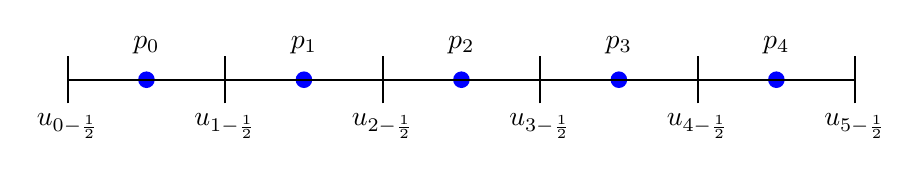
\begin{tikzpicture}[scale=1.0]
    \foreach \i in {0,...,5}{
      \draw[thick] (2*\i,-0.3) -- (2*\i,0.3);
      \node[below] at (2*\i,-0.3) {$u_{\i-\frac12}$};
    }
    \foreach \i in {0,...,4}{
      \fill[blue] (2*\i+1,0) circle (3pt);
      \node[above] at (2*\i+1,0.2) {$p_{\i}$};
    }
    \draw[thick] (0,0) -- (10,0);
  \end{tikzpicture}
  \end{center}
  \begin{itemize}
    \item $p$ at cell centers, $u$ at cell faces (Arakawa C in 2D): compact, accurate acoustic operator
    \[
      (\partial_x u)_j\approx\frac{u_{j+1/2}-u_{j-1/2}}{\Delta x},\qquad
      (\partial_x p)_{j+1/2}\approx\frac{p_{j+1}-p_j}{\Delta x}\quad(\text{2nd order}).
    \]
    \item Higher order: wider centered staggered stencils (4th/6th order) for $\LL$.
    \item \textbf{Advection} $\NN=-U\partial_x$: both fields must be advected on their own grid points
    $\Rightarrow$ high-order upwind-biased stencils (e.g.\ 3rd/5th order). With constant $U$ and the same stencil on both
    arrays, $\LL$ and $\NN$ are circulant and commute: the exact semi-discrete solution is known (used as reference below).
  \end{itemize}
\end{frame}

\begin{frame}{High-order advection operators}
  Upwind-biased reconstruction of face values $\hat\phi_{j+1/2}$ (for $U>0$), advective operator
  \[
    (\NN\phi)_j=-\frac{U}{\Delta x}\big(\hat\phi_{j+1/2}-\hat\phi_{j-1/2}\big).
  \]
  \begin{center}
  \begin{tabular}{ll}
    \toprule
    order & face reconstruction \\
    \midrule
    1st & $\hat\phi_{j+1/2}=\phi_j$\\
    3rd & $\hat\phi_{j+1/2}=\tfrac16\big(-\phi_{j-1}+5\phi_j+2\phi_{j+1}\big)$\\
    5th & $\hat\phi_{j+1/2}=\tfrac1{60}\big(2\phi_{j-2}-13\phi_{j-1}+47\phi_j+27\phi_{j+1}-3\phi_{j+2}\big)$\\
    \bottomrule
  \end{tabular}
  \end{center}
  \begin{itemize}
    \item Odd orders: built-in dissipation (upwinding) $\Rightarrow$ implicit damping of grid-scale noise.
    \item Time integrator error must stay below the spatial error: low-order splitting would spoil the high-order advection.
    \item Fourier symbol of the discrete operator: $\NN\to-\ii U\,\kappa(k\Delta x)/\Delta x$, used for analysis of all schemes above.
  \end{itemize}
\end{frame}

\begin{frame}{Test setup: 1D}
  \begin{itemize}
    \item Periodic domain $[0,L]$, background $U$, $c$ with $M=U/c\in\{0.05,0.1,0.3\}$.
    \item Smooth initial data: Gaussian pressure pulse (right/left moving acoustic waves + advection).
    \item Reference: exact semi-discrete solution (circulant operators commute: analytic in Fourier space).
    \item $L=1000$\,km, 400 cells, $c=350$\,m/s, $U=50$\,m/s; slow steps $h=50\to3$\,s ($ch/\Delta x=7\to0.4$).
    \item Study (all exponentials and $\ph$-functions from the fast integrator):
    \begin{enumerate}
      \item pressure pulse: out and back (Lawson-RK4, fast order 4),
      \item convergence in $h$ with the acoustic substep $\tau$ fixed (stability limited): fast order 2 vs.\ 4, Lawson-RK4 vs.\ ETDRK4,
      and the split-explicit RK3 of WRF (forward--backward, with and without pressure extrapolation),
      \item MIS methods (RK3, MIS-KW3, MIS54) and the linear acoustics stability test of Knoth--Wensch,
      \item work--precision: fast order 2, 4, 6 at large and at small slow steps.
    \end{enumerate}
  \end{itemize}
\end{frame}

\begin{frame}[fragile]{Julia: the fast integrator (\texttt{fast\_fb.jl}, abbreviated)}
\begin{lstlisting}
function kickA!(p, u, m, alpha, t, Gp)         # exact p-kick, time advances by alpha
    n = m.nx;  a = -alpha*m.rho*m.c^2/m.dx
    for j in 1:n
        d = 9/8*(u[wrap(j+1,n)] - u[j]) - 1/24*(u[wrap(j+2,n)] - u[wrap(j-1,n)])
        p[j] += a*d
    end
    for k in 1:length(Gp)                      # polynomial source: exact time integral
        w = ((t+alpha)^k - t^k)/factorial(k);  gk = Gp[k];  @. p += w*gk
    end
end                                            # kickB! (u-kick, t frozen) is analogous

function fast!(p, u, m, h, nsub, cf, Gp, Gu)   # (p,u) <- e^{hL}(p,u) + sum_k h^k phi_k(hL) G_k
    tau = h/nsub;  n = length(cf.b);  t = 0.0
    pend = cf.a[1]*tau
    for s in 1:nsub
        if s > 1;  pend += cf.a[1]*tau;  end   # merge neighbouring A-kicks
        for i in 1:n
            kickA!(p, u, m, pend, t, Gp);  t += pend
            kickB!(u, p, m, cf.b[i]*tau, t, Gu)
            pend = cf.a[i+1]*tau
        end
    end
    kickA!(p, u, m, pend, t, Gp)
end
\end{lstlisting}
  \vspace{-0.3em}
  \begin{itemize}\footnotesize
    \item \texttt{cf = Coeffs(order)} with \texttt{order} $\in\{2,4,6\}$; \texttt{Gp}, \texttt{Gu}: vectors of arrays $\mathbf G_1,\mathbf G_2,\dots$ (empty for a pure exponential).
  \end{itemize}
\end{frame}

\begin{frame}[fragile]{Julia: Lawson-RK4 step (4 evaluations of $\NN$, 4 applications of $E$)}
\begin{lstlisting}
function lawson_rk4_step!(p, u, m, h, nsub, cf, ws)
    fh = ws.fh
    E!(a, b) = fast_exp!(a, b, m, h/2, nsub, cf)                       # E = exp(hL/2)
    adv!(ws.ap, p, m, fh); adv!(ws.au, u, m, fh)                       # k1
    copyto!(ws.wp, p); copyto!(ws.wu, u); E!(ws.wp, ws.wu)             # w = E y
    @. ws.y2p = p + h/2 * ws.ap
    @. ws.y2u = u + h/2 * ws.au
    E!(ws.y2p, ws.y2u)                                                 # Y2 = E(y + h/2 k1)
    adv!(ws.bp, ws.y2p, m, fh); adv!(ws.bu, ws.y2u, m, fh)             # k2
    @. ws.tp = ws.wp + h/2 * ws.bp                                     # Y3 = w + h/2 k2
    @. ws.tu = ws.wu + h/2 * ws.bu
    adv!(ws.cp, ws.tp, m, fh); adv!(ws.cu, ws.tu, m, fh)               # k3
    @. ws.tp = ws.wp + h * ws.cp
    @. ws.tu = ws.wu + h * ws.cu
    E!(ws.tp, ws.tu)                                                   # Y4 = E(w + h k3)
    adv!(ws.ap, ws.tp, m, fh); adv!(ws.au, ws.tu, m, fh)               # k4
    @. ws.tp = ws.wp + (ws.y2p - ws.wp)/3 + h/3 * (ws.bp + ws.cp)
    @. ws.tu = ws.wu + (ws.y2u - ws.wu)/3 + h/3 * (ws.bu + ws.cu)
    E!(ws.tp, ws.tu)
    @. p = ws.tp + h/6 * ws.ap
    @. u = ws.tu + h/6 * ws.au
end
\end{lstlisting}
  \vspace{-0.3em}
  \begin{itemize}\footnotesize
    \item \texttt{adv!}: 5th order upwind flux form; all work arrays preallocated (\texttt{ws}); \texttt{etdrk4\_step!} has the same structure.
    \item Programs: \texttt{fast\_fb.jl} (module), \texttt{test\_fast.jl} (accuracy of $\ee^{h\LL},\ph_k$), \texttt{run\_experiments.jl} (data for the plots).
  \end{itemize}
\end{frame}

\begin{frame}{1D experiment: pressure pulse}
  \footnotesize
  $c=350$\,m/s, $U=50$\,m/s ($M=1/7$), $L=1000$\,km, 400 cells, $T=10^4$\,s: $(c+U)T=4L$ and $(c-U)T=3L$,
  so both acoustic pulses return to the start. Initial $p$: Gaussian, $u=0$. Lawson-RK4, $h=50$\,s ($ch/\Delta x=7$, $Uh/\Delta x=1$), fast integrator of order 4 with 8 substeps per $h/2$.
  \begin{center}
  \begin{tikzpicture}
    \begin{groupplot}[group style={group size=3 by 1,horizontal sep=0.7cm,y descriptions at=edge left},
        width=0.37\textwidth,height=4.0cm,xlabel={$x$ [km]},xmin=0,xmax=1000,ymin=-0.05,ymax=1.08,
        xtick={0,500,1000},ytick={0,0.5,1},grid=both,grid style={black!10},tick label style={font=\scriptsize},
        label style={font=\scriptsize},title style={font=\small}]
      \nextgroupplot[title={$t=0$},ylabel={pressure perturbation $p$}]
        \addplot[blue!70!black,very thick] table[col sep=comma,x=x_km,y=p0] {data_pressure_1d.csv};
      \nextgroupplot[title={$t=T/2$}]
        \addplot[black!45,dashed] table[col sep=comma,x=x_km,y=p0] {data_pressure_1d.csv};
        \addplot[blue!70!black,very thick] table[col sep=comma,x=x_km,y=p_half] {data_pressure_1d.csv};
      \nextgroupplot[title={$t=T$}]
        \addplot[black!45,dashed] table[col sep=comma,x=x_km,y=p0] {data_pressure_1d.csv};
        \addplot[blue!70!black,very thick] table[col sep=comma,x=x_km,y=p_T] {data_pressure_1d.csv};
    \end{groupplot}
  \end{tikzpicture}
  \end{center}
  \begin{itemize}
    \item $t=T/2$: the pulse has split into two half-amplitude pulses; the right-going one has traveled $2L$, the left-going one $1.5L$.
    \item $t=T$: back at the initial position; max.\ deviation $6\cdot10^{-6}$ (spatial dissipation of the upwind stencil plus time error).
  \end{itemize}
\end{frame}

\begin{frame}{Convergence in the slow step: why the fast integrator needs high order}
  \begin{columns}[T]
    \column{0.56\textwidth}
      \begin{tikzpicture}
        \begin{axis}[width=\textwidth,height=5.6cm,xmode=log,ymode=log,xlabel={slow step $h$ [s]},ylabel={max error of $p$ at $t=T$},
            grid=both,grid style={black!10},legend style={font=\scriptsize,draw=none,fill=none},legend pos=north west,
            xmin=2.5,xmax=62,xtick={3.125,6.25,12.5,25,50},xticklabels={3.1,6.3,12.5,25,50},minor tick num=0,
            tick label style={font=\scriptsize},label style={font=\small},ymin=1e-10,ymax=1e-2]
          \addplot[red!75!black,mark=square*,thick] table[col sep=comma,x=h,y=lawson_o2] {data_conv_1d.csv};
          \addlegendentry{Lawson-RK4, fast order 2}
          \addplot[blue!70!black,mark=*,thick] table[col sep=comma,x=h,y=lawson_o4] {data_conv_1d.csv};
          \addlegendentry{Lawson-RK4, fast order 4}
          \addplot[black!60!green,mark=triangle*,thick] table[col sep=comma,x=h,y=etdrk4_o4] {data_conv_1d.csv};
          \addlegendentry{ETDRK4, fast order 4}
          \addplot[black,dashed,domain=3:50,samples=2] {8.93e-13*x^4};
          \addlegendentry{$h^4$}
        \end{axis}
      \end{tikzpicture}
    \column{0.42\textwidth}
      \footnotesize
      \begin{itemize}
        \item Acoustic substep fixed by stability: $\tau=1.56$\,s, i.e.\ nsub $=16,8,4,2,1$ per $h/2$.
        \item \textbf{Fast order 2:} error stalls at $1.7\cdot10^{-6}$ for $h\lesssim25$\,s: the 4th order slow scheme cannot be exploited.
        \item \textbf{Fast order 4:} fourth order in $h$ from 50 down to 6\,s ($1.6\cdot10^{-9}$); at $h=3$\,s (nsub $=1$) its fast error shows ($4.5\cdot10^{-10}$).
        \item ETDRK4: same order, much larger error constant here ($1.6\cdot10^{-3}$ vs.\ $5.6\cdot10^{-6}$ at $h=50$\,s); the curve flattens at $h\approx3$\,s because of the fast error (nsub $=1$).
        \item $\LL,\NN$ commute in this test: Lawson is then very accurate; ETDRK4 may profit when they do not.
      \end{itemize}
  \end{columns}
\end{frame}

\begin{frame}{Split-explicit RK3 (WRF) on the same test}
  \begin{center}
  \begin{tikzpicture}
    \begin{groupplot}[group style={group size=2 by 1,horizontal sep=1.5cm},width=0.47\textwidth,height=4.9cm,
        grid=both,grid style={black!10},tick label style={font=\scriptsize},label style={font=\scriptsize},
        title style={font=\small},legend style={font=\scriptsize,draw=none,fill=white,fill opacity=0.8,text opacity=1},
        legend cell align=left]
      \nextgroupplot[title={convergence (max error of $p$ at $t=T$)},xmode=log,ymode=log,xlabel={slow step $h$ [s]},
          xmin=0.6,xmax=62,xtick={0.78125,3.125,12.5,50},xticklabels={0.78,3.1,12.5,50},minor tick num=0,
          ymin=1e-10,ymax=1]
        \addplot[blue!70!black,mark=*,thick] table[col sep=comma,x=h,y=lawson_o4] {data_conv_1d.csv};
        \addplot[black!60!green,mark=triangle*,thick] table[col sep=comma,x=h,y=etdrk4_o4] {data_conv_1d.csv};
        \addplot[orange!85!black,mark=diamond*,thick] table[col sep=comma,x=h,y=rk3_fb] {data_conv_1d.csv};
        \addplot[violet,mark=pentagon*,thick] table[col sep=comma,x=h,y=rk3_fb_pe] {data_conv_1d.csv};
        \addplot[orange!85!black,mark=diamond,thick,dashed] table[col sep=comma,x=h,y=rk3_fb] {data_conv_rk3.csv};
        \addplot[black,dashed,domain=0.7:14,samples=2] {4.1e-5*x^2};
        \node[blue!70!black,anchor=east,font=\scriptsize] at (axis cs:2.9,4.5e-10) {Lawson-RK4};
        \node[black!60!green,anchor=east,font=\scriptsize] at (axis cs:2.9,1.65e-7) {ETDRK4};
        \node[orange!85!black,anchor=east,font=\scriptsize] at (axis cs:2.9,5e-6) {RK3 split, FB};
        \node[violet,anchor=south,font=\scriptsize] at (axis cs:9,6e-2) {RK3 split, FB + p-extrap.};
        \node[orange!85!black,anchor=west,font=\scriptsize] at (axis cs:0.62,4e-3) {RK3 split, $\Delta\tau=0.2$\,s};
        \node[black,anchor=south east,font=\scriptsize] at (axis cs:0.9,8e-5) {$h^2$};
      \nextgroupplot[title={stability: $\max_k$ spectral radius},xlabel={slow step $h$ [s] \quad($\Delta\tau\le1.56$\,s)},
          xmin=0,xmax=80,ymin=0.95,ymax=2.4,legend pos=north west]
        \addplot[orange!85!black,thick] table[col sep=comma,x=h,y=rho_fb] {data_rk3_stab.csv};
        \addlegendentry{FB, WRF stage 1}
        \addplot[violet,thick] table[col sep=comma,x=h,y=rho_fb_pe] {data_rk3_stab.csv};
        \addlegendentry{FB+p-extr., WRF stage 1}
        \addplot[orange!85!black,thick,dashed] table[col sep=comma,x=h,y=rho_fb_uni] {data_rk3_stab.csv};
        \addlegendentry{FB, uniform stage 1}
        \addplot[violet,thick,dashed] table[col sep=comma,x=h,y=rho_fb_pe_uni] {data_rk3_stab.csv};
        \addlegendentry{FB+p-extr., uniform stage 1}
    \end{groupplot}
  \end{tikzpicture}
  \end{center}
  \vspace{-0.6em}
  \scriptsize
  \begin{itemize}
    \item Undamped FB: unstable for $h\ge19$\,s ($ch/\Delta x\ge2.7$) for both stage-1 variants. Pressure extrapolation ($\beta=0.1$) stabilizes up to
    $h=27.5$\,s with WRF's single stage-1 step ($c\,h/(3\Delta x)=1.3$), up to $h=66$\,s with $n_s/3$ small steps in stage 1.
    \item Second order in $h$ when the fast part is resolved (dashed: factor 4 per halving), as predicted by the $\sin(\theta/2)/(\theta/2)$ term. The dip at $h=3.1$\,s ($n_s=2$) is a cancellation.
    \item Pressure extrapolation damps the \emph{resolved} acoustic pulse: error $\propto\beta\Delta\tau$, it does not decrease with $h$.
    \item Equal cost at $h=12.5$\,s ($\approx50$ kick pairs per step): Lawson-RK4 (fast order 2) $2.6\cdot10^{-8}$, split-explicit RK3 $6.4\cdot10^{-3}$.
  \end{itemize}
\end{frame}

\begin{frame}{MIS methods on the 1D test}
  \begin{center}
  \begin{tikzpicture}
    \begin{groupplot}[group style={group size=2 by 1,horizontal sep=1.3cm},width=0.47\textwidth,height=4.9cm,
        xmode=log,ymode=log,xlabel={slow step $h$ [s]},grid=both,grid style={black!10},
        xmin=2.5,xmax=125,xtick={3.125,6.25,12.5,25,50,100},xticklabels={3.1,6.3,12.5,25,50,100},minor tick num=0,
        tick label style={font=\scriptsize},label style={font=\scriptsize},title style={font=\small},ymin=1e-10,ymax=1]
      \nextgroupplot[title={fast part (almost) exact},ylabel={max error of $p$ at $t=T$}]
        \addplot[orange!85!black,mark=diamond*,thick] table[col sep=comma,x=h,y=rk3ws_ex] {data_conv_mis.csv};
        \addplot[red!70!black,mark=square*,thick] table[col sep=comma,x=h,y=kw3_ex] {data_conv_mis.csv};
        \addplot[teal,mark=*,thick] table[col sep=comma,x=h,y=mis54_ex] {data_conv_mis.csv};
        \addplot[blue!70!black,mark=o,thick,densely dotted] table[col sep=comma,x=h,y=lawson_o4] {data_conv_1d.csv};
        \addplot[black,dashed,domain=3:15,samples=2] {2.5e-7*x^3};
        \addplot[black,dashed,domain=3:100,samples=2] {4e-10*x^4};
        \node[orange!85!black,anchor=south,font=\scriptsize] at (axis cs:12.5,1.5e-2) {RK3 (WS)};
        \node[red!70!black,anchor=north,font=\scriptsize] at (axis cs:5.3,6e-6) {MIS-KW3};
        \node[teal,anchor=north west,font=\scriptsize] at (axis cs:55,1.5e-4) {MIS54};
        \node[blue!70!black,anchor=west,font=\scriptsize] at (axis cs:14,1.5e-9) {Lawson-RK4 (fast o4)};
        \node[black,anchor=west,font=\scriptsize] at (axis cs:15.5,8.4e-4) {$h^3$};
        \node[black,anchor=south east,font=\scriptsize] at (axis cs:30,2e-3) {$h^4$};
      \nextgroupplot[title={fast integrator in the MIS stages ($\tau\le1.56$\,s)}]
        \addplot[teal,mark=*,thick] table[col sep=comma,x=h,y=mis54_ex] {data_conv_mis.csv};
        \addplot[teal,mark=triangle*,thick,dashed] table[col sep=comma,x=h,y=mis54_lf] {data_conv_mis.csv};
        \addplot[teal,mark=square,thick,dotted] table[col sep=comma,x=h,y=mis54_fb] {data_conv_mis.csv};
        \addplot[red!70!black,mark=triangle*,thick,dashed] table[col sep=comma,x=h,y=kw3_lf] {data_conv_mis.csv};
        \addplot[red!70!black,mark=square,thick,dotted] table[col sep=comma,x=h,y=kw3_fb] {data_conv_mis.csv};
        \node[black,anchor=south east,font=\scriptsize,align=right] at (axis cs:118,2e-10)
          {\textcolor{teal}{MIS54}, \textcolor{red!70!black}{MIS-KW3}\\ solid: exact fast part\\ dashed: leapfrog (symmetric, order 2)\\ dotted: WRF forward--backward};
    \end{groupplot}
  \end{tikzpicture}
  \end{center}
  \vspace{-0.6em}
  \scriptsize
  \begin{itemize}
    \item Orders 2, 3, 4 confirmed (MIS54: factor 16 per halving from $h=100$ to $3.1$\,s). MIS54 is stable for $h<99$\,s ($ch/\Delta x<13.9$)
    \emph{without} divergence damping; RK3 is unstable from $h=19.5$\,s, MIS-KW3 is weakly unstable already at small $h$ on this grid
    ($|\lambda|_{\max}-1=2\cdot10^{-6}$ at $h=6.25$\,s, $2\cdot10^{-3}$ at $12.5$\,s).
    \item The fast integrator must be symmetric and of high order: WRF's forward--backward step leaves an $\mathcal O(\tau)$ error that does not cancel between
    MIS stages (they start from combinations of earlier stages), leapfrog an $\mathcal O(\tau^2)$ error; they stall at $2\cdot10^{-4}$ and $5\cdot10^{-5}$.
    \item MIS54 has the fast work of RK3 ($\sum d_i=1.88$) but 5 evaluations of $\NN$; in this test (commuting $\LL$, $\NN$) Lawson-RK4 is still more accurate.
  \end{itemize}
\end{frame}

\begin{frame}{Example from Knoth--Wensch: stability regions for linear acoustics}
  \footnotesize
  $u_t+Uu_x=-c_s\Pi_x$, $\Pi_t+U\Pi_x=-c_su_x$ (Knoth--Wensch 2014, eq.\ (10)); C-grid, central differences for the acoustic terms,
  3rd order upwind advection; exact integration of the fast stages; $\max_k|\lambda(S(C_{\rm adv},C_{\rm sound},k))|$ over 40 Fourier modes.
  \begin{center}
  \begin{tikzpicture}
    \begin{groupplot}[group style={group size=3 by 1,horizontal sep=0.5cm,y descriptions at=edge left},width=0.37\textwidth,height=4.3cm,
        xmin=0,xmax=12,ymin=0,ymax=2.2,xlabel={$C_{\rm sound}=c_sh/\Delta x$},ylabel={$C_{\rm adv}=Uh/\Delta x$},
        tick label style={font=\scriptsize},label style={font=\scriptsize},title style={font=\small},
        colormap={stab}{color(0cm)=(red!18); color(1cm)=(blue!45)},point meta min=0,point meta max=1,axis on top]
      \nextgroupplot[title={RK3 (Wicker--Skamarock)}]
        \addplot[matrix plot*,mesh/ordering=y varies,mesh/rows=45,mesh/cols=61,point meta=explicit]
          table[col sep=comma,x=cs,y=ca,meta=rk3ws] {data_kw_stab.csv};
      \nextgroupplot[title={MIS-KW3}]
        \addplot[matrix plot*,mesh/ordering=y varies,mesh/rows=45,mesh/cols=61,point meta=explicit]
          table[col sep=comma,x=cs,y=ca,meta=kw3] {data_kw_stab.csv};
      \nextgroupplot[title={MIS54}]
        \addplot[matrix plot*,mesh/ordering=y varies,mesh/rows=45,mesh/cols=61,point meta=explicit]
          table[col sep=comma,x=cs,y=ca,meta=mis54] {data_kw_stab.csv};
    \end{groupplot}
  \end{tikzpicture}
  \end{center}
  \begin{itemize}
    \item Blue: stable. Pure advection ($C_{\rm sound}=0$): $C_{\rm adv}\le1.63$ for the 3-stage methods (RK3 with 3rd order upwinding), $2.06$ for MIS54.
    \item Without damping RK3 and MIS-KW3 become unstable for $C_{\rm sound}\gtrsim3$ and $\gtrsim2$ (exact fast part); MIS54 is stable on the whole range
    (checked with 400 modes), it was selected for this test.
    \item Same picture on our grid (4th order acoustics, 5th order upwind): MIS54 stable up to $ch/\Delta x=13.9$, RK3 only up to $2.7$.
  \end{itemize}
\end{frame}

\begin{frame}{Work--precision of the fast integrator (Lawson-RK4)}
  \begin{center}
  \begin{tikzpicture}
    \begin{groupplot}[group style={group size=2 by 1,horizontal sep=1.3cm},width=0.46\textwidth,height=5.0cm,xmode=log,ymode=log,
        xlabel={kick pairs per slow step ($4\times$nsub$\times$stages)},grid=both,grid style={black!10},
        tick label style={font=\scriptsize},label style={font=\scriptsize},title style={font=\small},
        legend style={font=\scriptsize,draw=none,fill=none}]
      \nextgroupplot[title={$h=50$\,s ($ch/\Delta x=7$)},ylabel={max error of $p$},ymin=1e-6,ymax=3e-4,legend pos=north east]
        \addplot[red!75!black,mark=square*,thick] table[col sep=comma,x=cost,y=err] {data_work_n200_o2.csv};
        \addlegendentry{order 2}
        \addplot[blue!70!black,mark=*,thick] table[col sep=comma,x=cost,y=err] {data_work_n200_o4.csv};
        \addlegendentry{order 4}
        \addplot[black!60!green,mark=triangle*,thick] table[col sep=comma,x=cost,y=err] {data_work_n200_o6.csv};
        \addlegendentry{order 6}
        \addplot[black,dashed] coordinates {(8,5.58e-6)(1400,5.58e-6)};
      \nextgroupplot[title={$h=12.5$\,s ($ch/\Delta x=1.75$)},ymin=1.5e-8,ymax=1e-4,legend pos=north east]
        \addplot[red!75!black,mark=square*,thick] table[col sep=comma,x=cost,y=err] {data_work_n800_o2.csv};
        \addplot[blue!70!black,mark=*,thick] table[col sep=comma,x=cost,y=err] {data_work_n800_o4.csv};
        \addplot[black!60!green,mark=triangle*,thick] table[col sep=comma,x=cost,y=err] {data_work_n800_o6.csv};
        \addplot[black,dashed] coordinates {(8,2.18e-8)(1400,2.18e-8)};
    \end{groupplot}
  \end{tikzpicture}
  \end{center}
  \footnotesize
  Dashed: error of Lawson-RK4 with exact $\ee^{h\LL/2}$ (slow-scheme error, the best possible).
  \begin{itemize}
    \item The fast integrator is accurate enough once its error is below the dashed line; missing points: substeps too large (unstable).
    \item The gain of a high-order fast integrator grows as the slow step (and tolerance) get smaller; order 6 does not pay off against the 4th order slow scheme.
  \end{itemize}
\end{frame}

\begin{frame}{Two dimensions}
  \[
    \partial_t\!\begin{pmatrix}p\\u\\v\end{pmatrix}
    =-\begin{pmatrix}\rho_0c^2(\partial_xu+\partial_yv)\\ \tfrac1{\rho_0}\partial_xp\\ \tfrac1{\rho_0}\partial_yp\end{pmatrix}
     -\big(U\partial_x+V\partial_y\big)\begin{pmatrix}p\\u\\v\end{pmatrix}.
  \]
  \begin{center}
  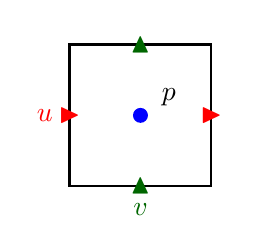
\begin{tikzpicture}[scale=0.9]
    \draw[thick] (0,0) rectangle (2,2);
    \fill[blue] (1,1) circle (3pt); \node at (1.4,1.25) {$p$};
    \node[red] at (0,1) {$\blacktriangleright$}; \node[red,left] at (-0.1,1) {$u$};
    \node[red] at (2,1) {$\blacktriangleright$};
    \node[black!60!green] at (1,0) {$\blacktriangle$}; \node[black!60!green,below] at (1,-0.1) {$v$};
    \node[black!60!green] at (1,2) {$\blacktriangle$};
  \end{tikzpicture}
  \end{center}
  \begin{itemize}
    \item Arakawa C-grid: $p$ at centers, $u$ on vertical faces, $v$ on horizontal faces.
    \item Advection of $u$ and $v$ requires \emph{different} stencils in $x$ and $y$; high-order upwind per direction.
    \item Fast operator $\LL$: 2D wave operator; $\ee^{h\LL}$, $\ph_k$ again by the substepping integrator (the FFT is only used for reference solutions).
    \item Tests: acoustic pulse in a uniform wind $(U,V)$; rotated wind to test directional splitting errors.
  \end{itemize}
\end{frame}

\begin{frame}{Expected observations (hypotheses to check)}
  \begin{itemize}
    \item Split-explicit (measured in 1D): the frozen slow forcing limits RK3 (WRF) to second order in $h$; without divergence damping it is
    unstable for $ch/\Delta x\gtrsim2.7$, pressure extrapolation stabilizes it but damps resolved acoustic signals.
    \item ETD/Lawson: acoustic stability for arbitrary $h$, order determined by the outer RK/ETD scheme.
    \item Resonance steps $ckh\approx 2\pi n$: visible spikes in the error for Lawson/ETD; reduced for averaging;
    removed for resonance-based schemes.
    \item When $[\LL,\NN]\neq0$ (variable wind, flux-form advection), the commutator gives the leading splitting error;
    averaging/resonance corrections remove it to higher order.
    \item In 2D: extra error from the directional splitting of $\NN$; cost advantage of FFT-based exponentials shrinks with non-periodic boundaries.
  \end{itemize}
  \vspace{0.5em}
  {\footnotesize (first item measured; the others to be checked with variable wind and in 2D)}
\end{frame}

% =====================================================================
\section{Summary}
% =====================================================================

\begin{frame}{Summary and outlook}
  \small
  \begin{itemize}
    \item The linear acoustic--advection system isolates the main stiffness/multirate difficulty of NWP dynamical cores.
    \item \textbf{Split-explicit} methods are ETD1-type methods with substepped approximations of $\ee^{h\LL}$ and $\ph_1(h\LL)$.
    \item \textbf{Lawson}, \textbf{averaging} and \textbf{resonance-based} methods treat the fast flow by an exponential and differ in how the
    slow interaction integral is approximated.
    \item One \textbf{high-order forward--backward (leapfrog/composition) integrator} delivers $\ee^{h\LL}$ and all $\ph_k$ through polynomial sources;
    its order must match the slow scheme because $\tau$ is stability limited.
    \item Application (staggered grid, 5th order upwind advection):
    \begin{itemize}\small
      \item Lawson-RK4 and ETDRK4 with a fast integrator of order 4: order 4 in $h$ up to $ch/\Delta x=7$; with order 2 the error stalls.
      \item Split-explicit RK3 (WRF): second order, divergence damping needed beyond $ch/\Delta x\approx2.7$, orders of magnitude less accurate at equal cost.
      \item MIS54: order 4, stable without damping up to $ch/\Delta x\approx14$, needs a symmetric high-order fast integrator in its stages.
    \end{itemize}
    \item Outlook: variable coefficients, orography/terrain-following coordinates, nonlinear (Euler) equations,
    IMEX/semi-implicit comparison, parallel efficiency; variable wind and 2D ($[\LL,\NN]\neq0$).
  \end{itemize}
  \vspace{0.5em}
  \centering\Large Thank you for your attention!
\end{frame}

% =====================================================================
\begin{frame}[allowframebreaks]{References (to be completed)}
  \footnotesize
  \begin{thebibliography}{99}
    \bibitem{KW78} J.\,B.\ Klemp, R.\,B.\ Wilhelmson, \emph{The simulation of three-dimensional convective storm dynamics}, J.\ Atmos.\ Sci.\ 35 (1978).
    \bibitem{WS02} L.\,J.\ Wicker, W.\,C.\ Skamarock, \emph{Time-splitting methods for elastic models using forward time schemes}, Mon.\ Wea.\ Rev.\ 130 (2002).
    \bibitem{KSD07} J.\,B.\ Klemp, W.\,C.\ Skamarock, J.\ Dudhia, \emph{Conservative split-explicit time integration methods for the compressible nonhydrostatic equations}, Mon.\ Wea.\ Rev.\ 135 (2007).
    \bibitem{Bal10} M.\ Baldauf, \emph{Linear stability analysis of Runge--Kutta-based partial time-splitting schemes for the Euler equations}, Mon.\ Wea.\ Rev.\ 138 (2010).
    \bibitem{KW14} O.\ Knoth, J.\ Wensch, \emph{Generalized split-explicit Runge--Kutta methods for the compressible Euler equations}, Mon.\ Wea.\ Rev.\ 142 (2014).
    \bibitem{BK21} T.\,P.\ Bauer, O.\ Knoth, \emph{Extended multirate infinitesimal step methods: Derivation of order conditions}, J.\ Comput.\ Appl.\ Math.\ 387 (2021) 112541.
    \bibitem{KWo98} O.\ Knoth, R.\ Wolke, \emph{Implicit-explicit Runge--Kutta methods for computing atmospheric reactive flows}, Appl.\ Numer.\ Math.\ 28 (1998).
    \bibitem{SR19} J.\,M.\ Sexton, D.\,R.\ Reynolds, \emph{Relaxed multirate infinitesimal step methods for initial-value problems}, arXiv:1808.03718 (2019).
    \bibitem{HO10} M.\ Hochbruck, A.\ Ostermann, \emph{Exponential integrators}, Acta Numerica 19 (2010).
    \bibitem{CM02} S.\,M.\ Cox, P.\,C.\ Matthews, \emph{Exponential time differencing for stiff systems}, J.\ Comput.\ Phys.\ 176 (2002).
    \bibitem{Law67} J.\,D.\ Lawson, \emph{Generalized Runge--Kutta processes for stable systems with large Lipschitz constants}, SIAM J.\ Numer.\ Anal.\ 4 (1967).
    \bibitem{WKG09} J.\ Wensch, O.\ Knoth, A.\ Galant, \emph{Multirate infinitesimal step methods for atmospheric flow simulation}, BIT 49 (2009).
    \bibitem{GP16} S.\ Gaudreault, J.\ Pudykiewicz, \emph{An efficient exponential time integration method for the numerical solution of the shallow water equations on the sphere}, J.\ Comput.\ Phys.\ 322 (2016).
  \end{thebibliography}
  {\scriptsize Please check the bibliographic details and add the specific references for averaging and resonance-based methods you intend to follow.}
\end{frame}

\end{document}
